\documentclass[12pt,letterpaper]{article}
\usepackage[spanish]{babel}
\usepackage[utf8]{inputenc}
\usepackage[T1]{fontenc}
\usepackage{graphicx}
\usepackage{listings}
\usepackage{xcolor}
\usepackage{enumerate}
\usepackage{fancyhdr}
\usepackage{float}
\usepackage{lastpage}
\usepackage{titling}
\usepackage{bookmark}
\usepackage{hyperref}

% Configuración para listings con soporte UTF-8
\lstset{
  basicstyle=\ttfamily\small,
  breaklines=true,
  extendedchars=true,
  inputencoding=utf8,
  showstringspaces=false,
  columns=flexible,
  literate={á}{{\'a}}1 {é}{{\'e}}1 {í}{{\'\i}}1 {ó}{{\'o}}1 {ú}{{\'u}}1
          {Á}{{\'A}}1 {É}{{\'E}}1 {Í}{{\'I}}1 {Ó}{{\'O}}1 {Ú}{{\'U}}1
          {ñ}{{\~n}}1 {Ñ}{{\~N}}1
}
\usepackage{amsmath}
\usepackage{float}
\usepackage{fancyhdr}
\usepackage{lastpage}
\usepackage{titling}

% Configuración del encabezado y pie de página
\setlength{\headheight}{50pt} % Aumentamos la altura del encabezado para el logo
\addtolength{\topmargin}{-35pt} % Ajustamos el margen superior
\pagestyle{fancy}
\fancyhf{}
\renewcommand{\headrulewidth}{1pt}
\renewcommand{\footrulewidth}{1pt}
\fancyhead[L]{
\includegraphics[height=35pt]{images/logo_uct.png}}
\fancyhead[R]{Programación~II}
\fancyfoot[C]{Página~\thepage}
\fancyfoot[R]{Octubre~2025}

% Aumentar el espacio superior del título
\setlength{\droptitle}{-4em}

% Configuración de colores y estilo para código
\definecolor{codegreen}{rgb}{0,0.6,0}
\definecolor{codegray}{rgb}{0.5,0.5,0.5}
\definecolor{codepurple}{rgb}{0.58,0,0.82}
\definecolor{backcolour}{rgb}{0.95,0.95,0.92}

\lstdefinestyle{mystyle}{
    backgroundcolor=\color{backcolour},   
    commentstyle=\color{codegreen},
    keywordstyle=\color{magenta},
    numberstyle=\tiny\color{codegray},
    stringstyle=\color{codepurple},
    basicstyle=\ttfamily\footnotesize,
    breakatwhitespace=false,         
    breaklines=true,                 
    captionpos=b,                    
    keepspaces=true,                 
    numbers=left,                    
    numbersep=5pt,                  
    showspaces=false,                
    showstringspaces=false,
    showtabs=false,                  
    tabsize=2
}

\lstset{style=mystyle}

\title{\textbf{Sistema de Gestión de Restaurante}\\
\large Evaluación 2 --- Programación II\\
\vspace{0.5cm}
\normalsize Universidad Católica de Temuco\\
\normalsize Facultad de Ingeniería\\
\normalsize Ingeniería Civil Informática}

\author{
    \textbf{Integrantes:}\\
    \vspace{0.3cm}
    Joaquin Carrasco Duran\\
    \vspace{0.3cm}
    Benjamin Cabrera\\
    \vspace{0.3cm}
    Leonardo Chavez\\
    \vspace{0.3cm}
    \textbf{Profesor:} Guido Mellado\\
    \vspace{0.3cm}
    \textbf{Asignatura:} Programación II\\
    \vspace{0.3cm}
    \textbf{Sección:} 2
}

\date{Octubre 2025}

\begin{document}

\maketitle
\newpage
\tableofcontents
\newpage

\section{Introducción}
Este informe presenta el desarrollo de un sistema de gestión para restaurantes implementado en Python. El sistema permite la administración de inventario, gestión de pedidos, generación de boletas y visualización de menús utilizando una interfaz gráfica moderna con customtkinter.

\section{Objetivos}
\subsection{Objetivo General}
Desarrollar un sistema de gestión integral para restaurantes que permita administrar inventario, pedidos y generación de documentos de manera eficiente.

\subsection{Objetivos Específicos}
\begin{itemize}
    \item Implementar un sistema de gestión de inventario para ingredientes
    \item Crear un sistema de pedidos con interfaz gráfica
    \item Desarrollar un generador de boletas automatizado
    \item Implementar visualización de menús en formato PDF
\end{itemize}

\section{Requerimientos Funcionales}

\subsection{Gestión de Inventario}
\begin{itemize}
    \item RF1: El sistema debe permitir agregar nuevos ingredientes al inventario
    \item RF2: El sistema debe permitir eliminar ingredientes existentes
    \item RF3: El sistema debe actualizar automáticamente las cantidades de ingredientes
    \item RF4: El sistema debe permitir cargar ingredientes desde archivos CSV
    \item RF5: El sistema debe validar la disponibilidad de ingredientes para menús
\end{itemize}

\subsection{Gestión de Pedidos}
\begin{itemize}
    \item RF6: El sistema debe permitir agregar ítems del menú al pedido actual
    \item RF7: El sistema debe permitir eliminar ítems del pedido actual
    \item RF8: El sistema debe calcular automáticamente el total del pedido
    \item RF9: El sistema debe verificar la disponibilidad de ingredientes al agregar ítems
    \item RF10: El sistema debe actualizar el inventario al confirmar un pedido
\end{itemize}

\subsection{Gestión de Menús}
\begin{itemize}
    \item RF11: El sistema debe mostrar el menú con imágenes representativas
    \item RF12: El sistema debe permitir generar una carta en formato PDF
    \item RF13: El sistema debe mostrar la disponibilidad de cada ítem del menú
    \item RF14: El sistema debe permitir visualizar el detalle de cada ítem
\end{itemize}

\subsection{Generación de Documentos}
\begin{itemize}
    \item RF15: El sistema debe generar boletas con un identificador único
    \item RF16: El sistema debe calcular automáticamente el IVA (19\%)
    \item RF17: El sistema debe almacenar las boletas generadas en una carpeta específica
    \item RF18: El sistema debe permitir visualizar las boletas generadas en formato PDF
\end{itemize}

\subsection{Interfaz de Usuario}
\begin{itemize}
    \item RF19: El sistema debe proporcionar una interfaz con pestañas para diferentes funcionalidades
    \item RF20: El sistema debe mostrar mensajes de confirmación para acciones importantes
    \item RF21: El sistema debe mostrar mensajes de error cuando ocurran problemas
    \item RF22: El sistema debe actualizar la interfaz en tiempo real al realizar cambios
\end{itemize}

\section{Arquitectura del Sistema}
El sistema está desarrollado siguiendo los principios de la programación orientada a objetos y utiliza varios patrones de diseño para mantener una estructura modular y mantenible.

\subsection{Patrones de Diseño Utilizados}
\begin{itemize}
    \item \textbf{Patrón Facade}: Implementado en la clase BoletaFacade para simplificar la generación de boletas.
    \item \textbf{Protocol (Interfaz moderna)}: Utilizado en IMenu para definir el contrato de los elementos del menú. Se implementa usando el módulo typing.Protocol de Python, que proporciona una forma más flexible y moderna de definir interfaces.

La implementación de IMenu utiliza Protocol en lugar de ABC (Abstract Base Class) para proporcionar un tipado estructural más flexible:

\begin{lstlisting}[language=Python, caption=Interfaz IMenu usando Protocol]
class IMenu(Protocol):
    """Interfaz para los elementos del menú utilizando tipado estructural."""
    nombre: str                        # Nombre del elemento del menú
    ingredientes: List[Ingrediente]    # Lista de ingredientes requeridos
    precio: float                      # Precio del elemento
    cantidad: int                      # Cantidad en el pedido
    icono_path: Optional[str]          # Ruta al ícono (opcional)
    
    def esta_disponible(self, stock: Stock) -> bool:
        """Verifica disponibilidad en el stock dado."""
        ...
\end{lstlisting}

Esta implementación con Protocol permite:
\begin{itemize}
    \item Tipado estructural: Las clases no necesitan declarar explícitamente que implementan IMenu
    \item Atributos tipados: Definición clara de tipos para cada atributo
    \item Compatibilidad implícita: Cualquier clase que tenga la estructura correcta es compatible
    \item Métodos abstractos: Define comportamiento requerido como \texttt{esta\_disponible()}
\end{itemize}
        \item \textbf{Composición sobre Herencia}: El sistema favorece la composición. Por ejemplo, la clase \texttt{CrearMenu} no hereda de \texttt{Ingrediente}, sino que "se compone de" una lista de objetos \texttt{Ingrediente}, lo que resulta en un diseño más flexible.
    
    \item \textbf{Factory (Fábrica Simple)}: La función \texttt{get\_default\_menus()} actúa como una fábrica que centraliza la creación de los objetos de menú iniciales.
    
    \item \textbf{Immutable Object (Objeto Inmutable)}: La clase \texttt{CrearMenu} es inmutable (\texttt{frozen=True}), lo que previene modificaciones accidentales y promueve una gestión de estado más segura.
    
    \item \textbf{Observer (Observador Implícito)}: La GUI se actualiza llamando a métodos como \texttt{actualizar\_treeview()} después de que los datos (el \texttt{Stock} o el \texttt{Pedido}) cambian, manteniendo la vista sincronizada con el modelo de datos.
\end{itemize}

\section{Diagrama de Clases}
\subsection{Estructura del Sistema}
\begin{figure}[H]
    \centering
    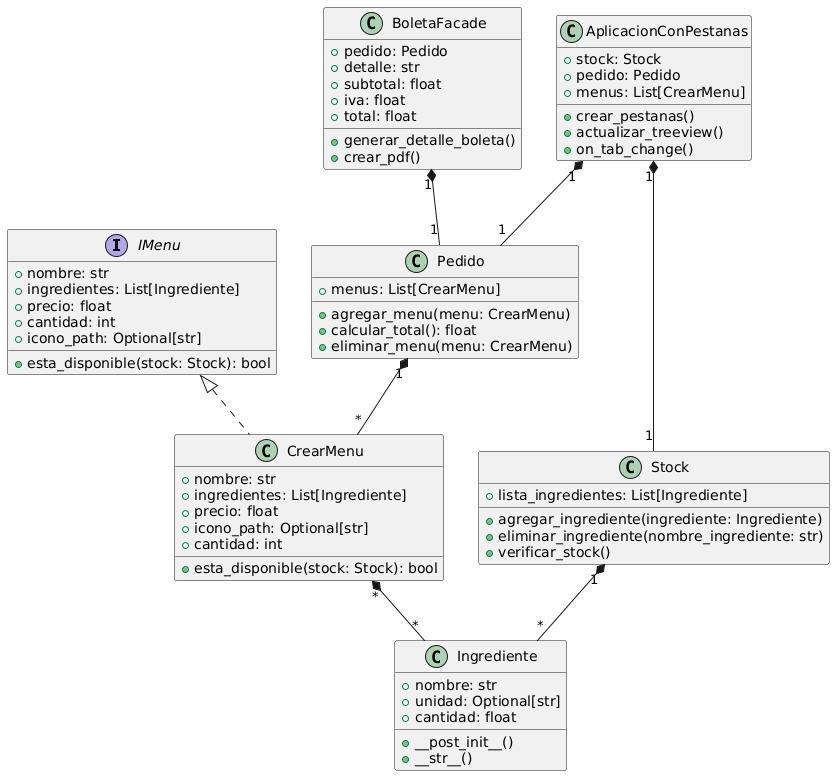
\includegraphics[width=\textwidth]{./images/diagrama.png}
    \caption{Diagrama de Clases del Sistema}\label{fig:diagrama}
\end{figure}
\clearpage %
\subsection{Explicación del Diagrama}
\begin{figure}[H]
    \centering
    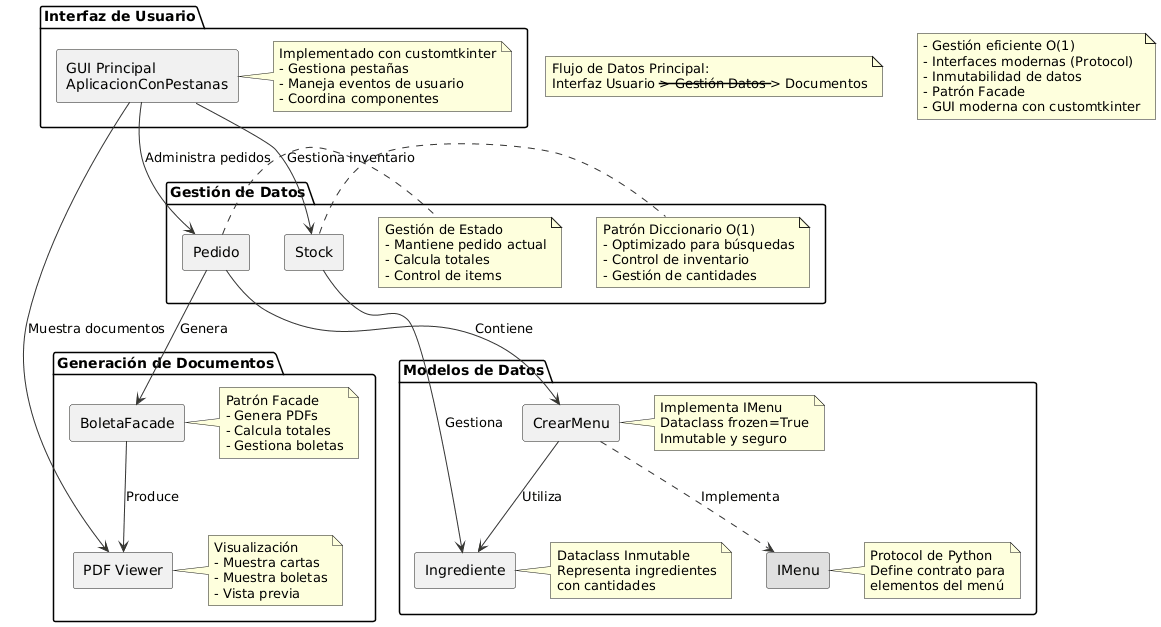
\includegraphics[width=0.9\textwidth]{./images/explicacion_diagrama.png}
    \caption{Explicación Detallada de las Relaciones entre Clases}\label{fig:explicacion-diagrama}
\end{figure}
\clearpage %

\subsection{Descripción de las Clases}
\begin{itemize}
    \item \textbf{AplicacionConPestanas}: Clase principal que coordina todas las funcionalidades del sistema.
    \item \textbf{Stock}: Gestiona el inventario de ingredientes.
    \item \textbf{Ingrediente}: Representa los ingredientes individuales.
    \item \textbf{CrearMenu}: Implementa la interfaz IMenu y representa los elementos del menú.
    \item \textbf{Pedido}: Maneja la gestión de pedidos.
    \item \textbf{BoletaFacade}: Simplifica la generación de boletas.
\end{itemize}

\section{Tecnologías Utilizadas}
\begin{itemize}
    \item \textbf{Python 3.13}: Lenguaje de programación principal
    \item \textbf{customtkinter}: Framework para la interfaz gráfica moderna
    \item \textbf{FPDF}: Biblioteca para generación de PDFs
    \item \textbf{PyMuPDF (fitz)}: Visualización de PDFs
    \item \textbf{Pandas}: Procesamiento de datos CSV
\end{itemize}

\section{Implementación}
\subsection{Gestión de Inventario}
El sistema maneja el inventario a través de la clase Stock, que utiliza un diccionario (de tipo Dict[str, Ingrediente]) como estructura de datos principal. Esta decisión de diseño garantiza un rendimiento óptimo con complejidad $O(1)$ para todas las operaciones principales:

\begin{itemize}
    \item Agregar nuevos ingredientes
    \item Eliminar ingredientes existentes
    \item Verificar disponibilidad
    \item Actualizar cantidades
\end{itemize}

A continuación, se muestra un ejemplo de la implementación del manejo de stock:

\begin{lstlisting}[language=Python, caption=Implementación de Stock]
class Stock:
    def __init__(self):
        self.lista_ingredientes: Dict[str, Ingrediente] = {}

    def agregar_ingrediente(self, ingrediente: Ingrediente):
        if ingrediente.nombre in self.lista_ingredientes:
            ing_existente = self.lista_ingredientes[ingrediente.nombre]
            nueva_cantidad = ing_existente.cantidad + ingrediente.cantidad
            ing_existente.cantidad = round(nueva_cantidad, 1)
        else:
            ingrediente.cantidad = round(ingrediente.cantidad, 1)
            self.lista_ingredientes[ingrediente.nombre] = ingrediente

    def verificar_ingredientes_suficientes(self, 
            ingredientes_necesarios: List[Ingrediente]) -> bool:
        for ing_necesario in ingredientes_necesarios:
            ing_stock = self.lista_ingredientes.get(ing_necesario.nombre)
            if ing_stock is None or ing_stock.cantidad < ing_necesario.cantidad:
                return False
        return True
\end{lstlisting}

\subsection{Sistema de Pedidos}
La gestión de pedidos se realiza mediante la clase Pedido, que ofrece:
\begin{itemize}
    \item Agregar elementos al pedido
    \item Calcular totales
    \item Verificar disponibilidad de ingredientes
    \item Generar boletas
\end{itemize}

\begin{lstlisting}[language=Python, caption=Implementación de Pedido]
class Pedido:
    def __init__(self):
        self.menus: Dict[str, CrearMenu] = {}
    
    def agregar_menu(self, menu: CrearMenu):
        if menu.nombre in self.menus:
            self.menus[menu.nombre].cantidad += menu.cantidad
        else:
            self.menus[menu.nombre] = menu
    
    def calcular_total(self) -> float:
        return sum(menu.precio * menu.cantidad 
                  for menu in self.menus.values())
\end{lstlisting}

\section{Interfaz Gráfica: Análisis por Pestaña}

\subsection{Configuración General de Pestañas}
El sistema utiliza un sistema de pestañas implementado con customtkinter para organizar las diferentes funcionalidades:

El siguiente código muestra la inicialización del sistema de pestañas. Se utiliza un enfoque modular donde cada pestaña se configura por separado, permitiendo una mejor organización del código y facilitando el mantenimiento. La numeración de las pestañas no es secuencial por motivos de desarrollo iterativo, pero esto no afecta la funcionalidad:

\begin{lstlisting}[language=Python, caption=Configuración de Pestañas]
def crear_pestanas(self):
    # Creación de pestañas en orden lógico de uso
    self.tab3 = self.tabview.add("Carga de ingredientes")  # Primer paso: cargar ingredientes
    self.tab1 = self.tabview.add("Stock")                  # Segundo paso: verificar stock
    self.tab4 = self.tabview.add("Carta restorante")       # Tercer paso: ver carta
    self.tab2 = self.tabview.add("Pedido")                 # Cuarto paso: hacer pedido
    self.tab5 = self.tabview.add("Boleta")                 # Paso final: generar boleta
    
    # Configuración individual de cada pestaña
    self.configurar_pestana1()                # Configura Stock
    self.configurar_pestana2()                # Configura Pedido
    self.configurar_pestana3()                # Configura Carga de ingredientes
    self._configurar_pestana_crear_menu()     # Configura Carta
    self._configurar_pestana_ver_boleta()     # Configura Boleta
\end{lstlisting}

\subsection{Pestaña: Carga de Ingredientes}
Esta pestaña permite dos métodos de ingreso de ingredientes\@: manual y por archivo CSV\@.

\subsubsection{Carga Manual}
La implementación de la carga manual de ingredientes incluye validaciones para asegurar la integridad de los datos. El sistema verifica que el nombre solo contenga letras y espacios, y que la cantidad sea un número válido. Además, se actualiza automáticamente la vista del inventario tras cada ingreso:

\begin{lstlisting}[language=Python, caption=Implementación de Carga Manual]
def ingresar_ingrediente(self):
    # Obtención de datos desde la interfaz
    nombre = self.entry_nombre.get()      # Nombre del ingrediente
    unidad = self.combo_unidad.get()      # Unidad de medida (g, kg, l, ml, etc.)
    cantidad = self.entry_cantidad.get()   # Cantidad del ingrediente

    # Validaciones de datos
    if not self.validar_nombre(nombre) or not self.validar_cantidad(cantidad):
        return  # Si no pasa las validaciones, se detiene el proceso

    # Creación y almacenamiento del ingrediente
    ingrediente = Ingrediente(nombre=nombre, unidad=unidad, cantidad=float(cantidad))
    self.stock.agregar_ingrediente(ingrediente)
    self.actualizar_treeview()  # Actualización de la interfaz
\end{lstlisting}

\subsubsection{Carga por CSV}
La carga masiva de ingredientes se realiza mediante archivos CSV, lo que permite una importación eficiente de datos. El sistema utiliza pandas para el procesamiento del archivo y maneja posibles errores de forma elegante, mostrando mensajes informativos al usuario:

\begin{lstlisting}[language=Python, caption=Implementación de Carga CSV]
def cargar_csv(self):
    # Apertura del diálogo de selección de archivo
    filename = filedialog.askopenfilename(
        title="Seleccionar archivo CSV",
        filetypes=[("CSV files", "*.csv")]  # Solo permite archivos CSV
    )
    if filename:
        try:
            # Lectura del archivo CSV usando pandas
            df = pd.read_csv(filename)
            
            # Procesamiento de cada fila del archivo
            for _, row in df.iterrows():
                # Creación de objeto Ingrediente desde datos CSV
                ingrediente = Ingrediente(
                    nombre=row['nombre'],     # Nombre del ingrediente
                    unidad=row['unidad'],     # Unidad de medida
                    cantidad=float(row['cantidad'])  # Cantidad convertida a float
                )
                # Agregado al inventario
                self.stock.agregar_ingrediente(ingrediente)
            
            self.actualizar_treeview()  # Actualización de la interfaz
        except Exception as e:
            # Manejo de errores con mensaje visual
            CTkMessagebox(title="Error", 
                message=f"Error al cargar el archivo: {str(e)}", 
                icon="warning")
\end{lstlisting}

\subsection{Pestaña: Stock}
Muestra y gestiona el inventario actual de ingredientes.

La clase Stock implementa un sistema eficiente de gestión de inventario utilizando un diccionario como estructura de datos principal\@. Esta decisión de diseño permite acceso $O(1)$ a los ingredientes y simplifica las operaciones de verificación y actualización. La clase incluye validaciones para evitar stocks negativos y manejo de ingredientes inexistentes:

\begin{lstlisting}[language=Python, caption=Gestión de Stock]
class Stock:
    def __init__(self):
        # Diccionario para acceso O(1) a ingredientes
        self.lista_ingredientes: Dict[str, Ingrediente] = {}

    def verificar_ingredientes_suficientes(self, ingredientes: List[Ingrediente]) -> bool:
        """
        Verifica si hay suficiente stock para una lista de ingredientes.
        Retorna False si falta algún ingrediente o la cantidad es insuficiente.
        """
        for ingrediente in ingredientes:
            ing_stock = self.lista_ingredientes.get(ingrediente.nombre)
            if not ing_stock or ing_stock.cantidad < ingrediente.cantidad:
                return False  # Ingrediente no existe o cantidad insuficiente
        return True  # Todos los ingredientes están disponibles

    def reservar_ingredientes(self, ingredientes: List[Ingrediente]):
        """
        Descuenta las cantidades del stock para los ingredientes usados.
        Solo se llama después de verificar_ingredientes_suficientes().
        """
        for ingrediente in ingredientes:
            ing_stock = self.lista_ingredientes[ingrediente.nombre]
            ing_stock.cantidad -= ingrediente.cantidad  # Actualización atómica
\end{lstlisting}

\subsection{Pestaña: Carta Restaurante}
Permite generar y visualizar la carta del restaurante en formato PDF\@.

La generación de la carta en PDF combina la creación del documento con su visualización inmediata. El sistema utiliza un visor de PDF personalizado (CTkPDFViewer) que permite una experiencia integrada y fluida para el usuario:

\begin{lstlisting}[language=Python, caption=Generación de Carta PDF]
def generar_y_mostrar_carta_pdf(self):
    try:
        # Configuración del archivo de salida
        pdf_path = "carta.pdf"
        
        # Generación del PDF con formato personalizado
        create_menu_pdf(
            self.menus,              # Lista de elementos del menú
            pdf_path,                # Ruta de salida
            titulo_negocio="Restaurante",
            subtitulo="Carta Primavera 2025",
            moneda="$"               # Símbolo monetario personalizable
        )
        
        # Limpieza del visor anterior si existe
        if self.pdf_viewer_carta is not None:
            self.pdf_viewer_carta.pack_forget()
        
        # Creación del nuevo visor con ruta absoluta
        self.pdf_viewer_carta = CTkPDFViewer(
            self.pdf_frame_carta,    # Contenedor del visor
            file=os.path.abspath(pdf_path)  # Ruta absoluta para evitar errores
        )
        # Configuración de expansión del visor
        self.pdf_viewer_carta.pack(expand=True, fill="both")
        
    except Exception as e:
        # Manejo de errores con interfaz gráfica
        CTkMessagebox(
            title="Error",
            message=f"Error al generar la carta: {str(e)}",
            icon="warning"
        )
\end{lstlisting}

\subsection{Pestaña: Pedido}
Gestiona la creación y modificación de pedidos actuales.

La clase Pedido gestiona la lógica de los pedidos activos, implementando un sistema que permite acumular cantidades de menús iguales y calcular totales de forma eficiente. Utiliza un diccionario para mantener la unicidad de los menús y facilitar las actualizaciones:

\begin{lstlisting}[language=Python, caption=Gestión de Pedidos]
class Pedido:
    def __init__(self):
        # Diccionario que mapea nombres de menús a objetos CrearMenu
        self.menus: Dict[str, CrearMenu] = {}

    def agregar_menu(self, menu: CrearMenu):
        """
        Agrega un menú al pedido o incrementa su cantidad si ya existe.
        Mantiene la consistencia de datos evitando duplicados.
        """
        if menu.nombre in self.menus:
            # Si el menú ya existe, solo incrementamos la cantidad
            self.menus[menu.nombre].cantidad += menu.cantidad
        else:
            # Si es nuevo, lo agregamos al diccionario
            self.menus[menu.nombre] = menu

    def calcular_total(self) -> float:
        """
        Calcula el total del pedido usando comprensión de listas.
        Multiplica el precio unitario por la cantidad de cada menú.
        """
        return sum(menu.precio * menu.cantidad 
                  for menu in self.menus.values())
\end{lstlisting}

\subsection{Pestaña: Boleta}
Genera y muestra las boletas de los pedidos.

La generación de boletas se implementa utilizando el patrón Facade para simplificar la compleja tarea de crear documentos PDF. La clase BoletaFacade encapsula toda la lógica de formato, cálculos y generación del archivo, proporcionando una interfaz simple para el cliente:

\begin{lstlisting}[language=Python, caption=Generación de Boletas]
class BoletaFacade:
    def generar_boleta(self):
        """
        Implementación del patrón Facade para la generación de boletas.
        Coordina todos los aspectos de la creación del PDF.
        """
        # Genera los detalles y cálculos previos
        self.generar_detalle_boleta()
        
        # Inicialización del documento PDF
        pdf = FPDF()
        pdf.add_page()
        pdf.set_font("Arial", size=12)
        
        # Configuración y generación del encabezado
        pdf.set_font("Arial", 'B', 16)
        pdf.cell(0, 10, "Boleta Restaurante", ln=True, align='L')
        
        # Generación de la tabla de detalles
        pdf.set_font("Arial", 'B', 12)
        for item in self.pedido.menus.values():
            subtotal = item.precio * item.cantidad
            # Formato tabular con bordes
            pdf.cell(70, 10, item.nombre, border=1)        # Nombre del ítem
            pdf.cell(20, 10, str(item.cantidad), border=1) # Cantidad
            pdf.cell(35, 10, f"${item.precio:.2f}", border=1)    # Precio unitario
            pdf.cell(30, 10, f"${subtotal:.2f}", border=1)       # Subtotal
            pdf.ln()  # Nueva línea
        
        # Sección de totales alineada a la derecha
        pdf.cell(120, 10, "Total:", 0, 0, 'R')
        pdf.cell(30, 10, f"${self.total:.2f}", ln=True, align='R')
        
        # Generación del archivo con nombre único
        timestamp = datetime.now().strftime("%Y%m%d_%H%M%S")
        pdf_filename = f"boleta_{timestamp}.pdf"  # Nombre único con timestamp
        pdf_path = os.path.join("boletas", pdf_filename)
        pdf.output(pdf_path)
        return pdf_path  # Retorna la ruta para visualización
\end{lstlisting}

\subsection{Componentes de la Interfaz}
La interfaz utiliza varios elementos modernos de customtkinter:

\subsubsection{Elementos Visuales}
\begin{itemize}
    \item Tarjetas de menú con íconos personalizados
    \item Visor de PDF integrado para cartas y boletas
    \item Tablas interactivas para gestión de datos
\end{itemize}

\subsubsection{Características Avanzadas}
\begin{itemize}
    \item Validación en tiempo real de ingredientes
    \item Actualización automática de stock
    \item Previsualización de documentos PDF
\end{itemize}

\subsection{Diseño Responsivo}
La interfaz se adapta dinámicamente al contenido y ofrece:
\begin{itemize}
    \item Diseño moderno con temas claro/oscuro
    \item Feedback visual en interacciones
    \item Mensajes de error y confirmación contextuales
    \item Organización jerárquica de información
\end{itemize}

\section{Conclusiones}
El sistema desarrollado cumple con los objetivos planteados, proporcionando una solución integral para la gestión de restaurantes. La implementación de patrones de diseño modernos como Protocol y principios de programación orientada a objetos permite una estructura mantenible y extensible. El uso de estructuras de datos optimizadas, como diccionarios para el manejo de inventario, asegura un rendimiento eficiente incluso con grandes volúmenes de datos.

Las decisiones de diseño tomadas, como:
\begin{itemize}
    \item El uso de typing.Protocol para interfaces modernas
    \item La implementación de diccionarios para operaciones $O(1)$ en el stock
    \item La aplicación del patrón Facade para simplificar operaciones complejas
    \item La utilización de customtkinter para una interfaz gráfica moderna
\end{itemize}

Han resultado en un sistema robusto, eficiente y fácil de mantener que cumple con los requisitos del proyecto y permite futuras extensiones.

\section{Anexos}
\subsection{Código Fuente}
A continuación se presentan fragmentos relevantes del código:

\begin{lstlisting}[language=Python, caption=Implementación de BoletaFacade]
class BoletaFacade:
    def __init__(self, pedido):
        self.pedido = pedido
        self.detalle = ""
        self.subtotal = 0
        self.iva = 0
        self.total = 0

    def generar_detalle_boleta(self):
        self.detalle = ""
        for item in self.pedido.menus:
            subtotal = item.precio * item.cantidad
            self.detalle += f"{item.nombre:<30} {item.cantidad:<10} ${item.precio:<10.2f} ${subtotal:<10.2f}\n"
        
        self.subtotal = self.pedido.calcular_total()
        self.iva = self.subtotal * 0.19
        self.total = self.subtotal + self.iva
\end{lstlisting}

\end{document}